% Exemplo de dissertação do INF-UFG com texto em portugues formatado com LaTeX
\documentclass[dissertacao]{inf-ufg}
% Opções da classe inf-ufg (ao usar mais de uma, separe por vírgulas)
%   [tese]         -> Tese de doutorado.
%   [dissertacao]  -> Dissertação de mestrado (padrão).
%   [monografia]   -> Monografia de especialização.
%   [relatorio]    -> Relatório final de graduação.
%   [abnt]         -> Usa o estilo "abnt-alf" de citação bibliográfica.
%   [nocolorlinks] -> Os links de navegação no texto ficam na cor preta.
%                     Use esta opção para gerar o arquivo para impressão
%                     da versão final do seu texto!!!
\usepackage[brazilian]{babel}
\usepackage[utf8]{inputenc}
\usepackage{multirow}
\usepackage[alf]{abntex2cite}
\usepackage{pgfgantt}
\usepackage{longtable}
\usepackage{mathtools}
\usepackage{float}
\usepackage{flushend}
\usepackage{amsmath}
\usepackage{subfig}
\usepackage{graphicx}
%----------------------------------------------------- INICIO DO DOCUMENTO %
\begin{document}

%------------------------------------------ AUTOR, TÍTULO E DATA DE DEFESA %
\autor{\textless Nome do Autor do Trabalho\textgreater} % (José da Silva)
\autorR{\textless Nome Reverso do Autor do Trabalho\textgreater} % (da Silva, José)

\titulo{\textless Título do Trabalho\textgreater}
\subtitulo{\textless Subtítulo do Trabalho\textgreater}

\cidade{\textless Cidade\textgreater} % Nome da cidade em foi desenvolvido o trabalho
\dia{\textless Dia\textgreater} %
\mes{\textless Mês\textgreater} % Data da apresentação/defesa do trabalho
\ano{\textless Ano\textgreater} % Formato numérico: \dia{01}, \mes{01} e \ano{2009}

%-------------------------------------------------------------- ORIENTADOR %
\orientador{\textless Nome do Orientador\textgreater}
\orientadorR{\textless Nome Reverso do Orientador\textgreater}
% Use os comandos a seguir se for Orientadora e nao Orientador.
%\orientadora{\textless Nome da Orientadora\textgreater}
%\orientadoraR{\textless Nome Reverso da Orientadora\textgreater}

\coorientador{\textless Nome do Co-orientador\textgreater}
\coorientadorR{\textless Nome Reverso do Co-orientador\textgreater}
% Use os comandos a seguir se for Co-orientadora e nao Coorientador.
%\coorientadora{\textless Nome da Co-orientadora\textgreater}
%\coorientadoraR{\textless Nome Reverso da Co-orientadora\textgreater}

%-------------------------------------------------- INSTITUIÇÃO E PROGRAMA %
\universidade{\textless Nome da Universidade\textgreater} % {Universidade Federal de Goiás}
\uni{\textless Sigla da Universidade\textgreater}         % UFG
\unidade{\textless Nome da Unidade Acadêmica\textgreater} %Instituto de Informática
\departamento{\textless Nome do Departamento\textgreater} %Unidades com mais de um depto.

\universidadeco{\textless Nome da Universidade do Co-orientador\textgreater}
\unico{\textless Sigla da Universidade do Co-orientador\textgreater}
\unidadeco{\textless Nome da Unidade Acadêmica do Co-orientador\textgreater}

\programa{\textless Nome do Programa de Pós-Graduação\textgreater} % Computação
\concentracao{\textless Área de Concentração\textgreater}

%-------------------------------------------------- ELEMENTOS PRÉ-TEXTUAIS %
\capa    % Gera o modelo da capa externa do trabalho
\publica % Gera a autorização para publicação em formato eletrônico
\rosto   % Primeira folha interna do trabalho

\begin{aprovacao}
\banca{\textless Nome do membro da banca\textgreater}{\textless Unidade acadêmica\textgreater\ -- \textless Sigla da universidade\textgreater}
% Use o comando \profa se o membro da banca for do sexo feminino.
\profa{\textless Nome do membro da banca\textgreater}{\textless Unidade acadêmica\textgreater\ -- \textless Sigla da universidade\textgreater}
\end{aprovacao}
\direitos{\textless Texto com um perfil resumido do autor do trabalho. Por exemplo: (Graduou--se em Artes Cênicas na UFG - Universidade Federal de Goiás. Durante sua graduação, foi monitor no departamento de Filosofia da UFG e pesquisador do CNPq em um trabalho de iniciação científica no departamento de Biologia. Durante o Mestrado, na USP - Universidade de São Paulo, foi bolsista da FAPESP e desenvolveu um trabalho teórico na resolução do Problema das Torres de Hanói. Atualmente desenvolve soluções para problemas de balanceamento de ração para a pecuária de corte.)\textgreater}

\begin{dedicatoria}
\textless Dedicatória do trabalho a alguma pessoa, entidade, etc.\textgreater
\end{dedicatoria}
\begin{agradecimentos}
\textless Texto com agradecimentos àquelas pessoas/entidades que, na opinião do autor, deram alguma contribuíção relevante para o desenvolvimento do trabalho.\textgreater
\end{agradecimentos}


\epigrafe{\textless Epígrafe é uma citação relacionada com o tópico do texto\textgreater}
{\textless Nome do autor da citação\textgreater}
{\textless Título da referência à qual a citação pertence\textgreater}
\chaves{\textless Palavra chave 1, palavra chave 2, etc.\textgreater}

\begin{resumo} 
\textless Resumo do trabalho\textgreater
\end{resumo}

\keys{\textless Keyword 1, keyword 2, etc.\textgreater}

\begin{abstract}{\textless Work title\textgreater}
A sketchy summary of the main points of the text.
\end{abstract}

\tabelas[figtabalgcod]
%Opções:
%nada [] -> Gera apenas o sumário
%fig     -> Gera o sumário e a lista de figuras
%tab     -> Sumário e lista de tabelas
%alg     -> Sumário e lista de algoritmos
%cod     -> Sumário e lista de códigos de programas
%
% Pode-se usar qualquer combinação dessas opções.
% Por exemplo:
%  figtab       -> Sumário e listas de figuras e tabelas
%  figtabcod    -> Sumário e listas de figuras, tabelas e
%                  códigos de programas
%  figtabalg    -> Sumário e listas de figuras, tabelas e algoritmos
%  figtabalgcod -> Sumário e listas de figuras, tabelas, algoritmos e
%                  códigos de programas

%--------------------------------------------------------------- CAPÍTULOS %

\chapter{Introdução}
\label{cap:intro}

Este documento mostra como usar o \LaTeX\ com a classe \textsf{inf-ufg} para formatar teses, dissertações, monografias e relatórios de conclusão de curso, segundo o padrão adotado pelo Instituto de Informática da UFG. Este documento e a classe \textsf{inf-ufg} foram, em grande parte, copiados e adaptados da classe \textsf{thesisPUC} e do texto de Thomas Lewiner \cite{Lew2002} que descreve a sua utilização.

 \LaTeX\ é um sistema de editoração eletrônica muito usado para produzir documentos científicos de alta qualidade tipográfica. O sistema também é útil para produzir todos os tipos de outros documentos, desde simples cartas até livros completos.

Se você precisar de algum material de apoio referente ao \LaTeX, dê uma olhada em um dos sites do Comprehensive TEX Archive Network (CTAN). O site está em \href{http://www.ctan.org/}{www.ctan.org}. Todos os pacotes podem ser obtidos via \textsf{FTP} \href{ftp://www.ctan.org/}{ftp://www.ctan.org} e existem vários servidores em todo o mundo. Eles podem ser encontrados, por exemplo, em \href{ftp://ctan.tug.org/}{ftp://ctan.tug.org} (EUA), \href{ftp://ftp.dante.de/}{ftp://ftp.dante.de} (Alemanha), \href{ftp://ftp.tex.ac.uk/}{ftp://ftp.tex.ac.uk} (Reino Unido).

Você pode encontrar uma grande quantidade de informações e dicas na página dos usuários brasileiros de \LaTeX\ (\TeX-BR). O endereço é \href{http://biquinho.furg.br/tex-br/}{http://biquinho.furg.br/tex-br/}.
Tanto no CTAN quanto no \TeX-BR estão disponíveis bons documentos em português sobre o \LaTeX. Em particular no CTAN, está disponível uma introdução bastante completa em português: \href{http://www.ctan.org/tex-archive/info/lshort/portuguese-BR/lshortBR.pdf}{CTAN:/tex-archive/info/lshort/portuguese-BR/}. No \TeX-BR também existe um documento com exemplos de uso de \LaTeX\ e de vários pacotes: \href{http://biquinho.furg.br/tex-br/doc/LaTeX-demo/}{http://biquinho.furg.br/tex-br/doc/LaTeX-demo/} . O objetivo é ser, através de exemplos, um guia para o usuário de \LaTeX\ iniciante e intermediário, podendo, ainda, servir como um guia de referência rápida para usuários avançados.

Se você quer usar o \LaTeX\ em seu computador, verifique em quais sistemas ele está disponível em \href{http://www.ctan.org/tex-archive/systems/}{CTAN:/tex-archive/systems}. Em particular para \textsf{MS Windows}, o sistema gratuito \href{http://www.miktex.org/}{MikTeX}, disponível no CTAN e no site \href{http://www.miktex.org/}{www.miktex.org} é completo e atualizado de todas as opções  que você poderia precisar para editar o seu texto.

O estilo \textsf{inf-ufg} se integra completamente ao \LaTeXe. Uma tese, dissertação ou monografia escrita no estilo padrão do \LaTeX\ para teses (estilo \verb|report|) pode ser formatada em 15 minutos para se adaptar às normas da UFG.

O estilo \textsf{inf-ufg} foi desenhado para minimizar a quantidade de texto e de comandos necessários para escrever a sua dissertação. Só é preciso inserir algumas macros no início do seu arquivo \LaTeX, precisando os dados bibliográficos da sua dissertação (por exemplo o seu nome, o titulo da dissertação\ldots). Em seguida, cada página dos elementos pré-textuais será formatada usando macros ou ambientes específicos. O corpo do texto é editado normalmente. Finalmente, as referências bibliográficas podem ser entradas manualmente (via o comando \verb|\bibitem| do \LaTeX\ padrão) ou usando o sistema BiBTeX (muito mais recomendável). Neste caso, os arquivos \verb|inf-ufg.bst| e \verb|abnt-alf.bst| permitem a formatação das referências bibliográficas segundo as normas da UFG.

\chapter{Descrição da classe \textsf{inf-ufg}}
\label{cap:descr}

%% - - - - - - - - - - - - - - - - - - - - - - - - - - - - - - - - - - -
\section{Opções da classe}
\label{sec:opcoes}
Para usar esta classe num documento \LaTeXe, coloque os arquivos 
\verb|inf-ufg.cls|,\ \verb|inf-ufg.bst|,\ \verb|abnt-num.bst|,\ \verb|atbeginend.sty|\ e \verb|tocloft.sty|\ numa pasta onde o compilador \LaTeX\ pode achá--lo (normalmente na mesma pasta que seu arquivo \verb|.tex|), e defina--o como o estilo do seu documento. Por exemplo, uma dissertação de mestrado que usa o modelo abnt de citações bibliográficas:
\begin{verbatim}
\documentclass[dissertacao,abnt]{inf-ufg}
...
\begin{document}
\end{verbatim}

As opções da classe são \verb|[tese]| (para tese de doutorado), \verb|[dissertacao]| (para dissertação de mestrado), \verb|[monografia]| (para monografia de curso de especialização e \verb|[relatorio]| (para relatório final de curso de graduação). Se nenhuma opção for declarada, o documento é considerado como uma dissertação de mestrado. Se a opção \verb|[abnt]| for utilizada, as citações bibliográficas serão geradas conforme definido pelo grupo de trabalho \textsf{abnt-tex}. Contudo, o mais recomendável é não utilizar essa opção. Com a opção \verb|[nocolorlinks]| todos os {\em links} de navegação no texto ficam na cor preta. O ideal é usar esta opção para gerar o arquivo para impressão, pois a qualidade da impressão dos {\em links} fica superior.


%% - - - - - - - - - - - - - - - - - - - - - - - - - - - - - - - - - - -
\section{Parâmetros da classe}
\label{sec:param}
Os elementos pré-textuais são definidos página por página e dependem da correta definição dos parâmetros listados a seguir (aqueles que contém um texto/valor padrão não precisam ser definidos, caso atenda a situação do autor do texto que está usando a classe \verb|inf-ufg.cls|):

% \setlength{\topsep}{5.2em}
 \begin{itemize}%\addtolength{\itemsep}{-0.7em}
\item \verb|\autor| : Nome completo do autor da tese, começando pelo apelido (ex.: José da Silva);
\item \verb|\autorR| : Nome completo do autor da tese, começando pelo nome (ex.: da Silva, José);
\item \verb|\titulo| : Título da tese, dissertação, monografia ou relatório de conclusão de curso;
\item \verb|\subtitulo| : Se tiver um subtítulo, use este macro para defini--lo;

\item \verb|\cidade| : A cidade de edição. A cidade padrão é \textsf{Goiânia}.
\item \verb|\dia| : Dia do mês da data de defesa (1--31);
\item \verb|\mes| : Mês da data de defesa (1--12);
\item \verb|\ano| : Ano da data de defesa;

\item \verb|\universidade| : Nome completo da universidade. O nome padrão é \textsf{Universidade Federal de Goiás};
\item \verb|\uni| : Sigla da universidade. A sigla padrão é \textsf{UFG};
\item \verb|\unidade| : Nome da unidade acadêmica. O padrão é \textsf{Instituto de Informática};
\item \verb|\departamento| : Nome do departamento, com maiúscula na primeira letra (para o caso de unidades com mais de um departamento);

\item \verb|\programa| : Nome do programa de pós-graduação, com maiúscula na primeira letra. O padrão é \textsf{Computação};
\item \verb|\concentracao| : Nome da área de concentração;

\item \verb|\orientador| : Nome completo do orientador, começando pelo apelido;
\item \verb|\orientadorR| : Nome completo do orientador, começando pelo nome;

\item \verb|\orientadora| : Nome completo da orientadora, começando pelo apelido; use este comando e o próximo se for orientadora e nao orientador.
\item \verb|\orientadoraR| : Nome completo do orientadora, começando pelo nome;

% \item \verb|\CDU| : CDU das publicações do instituto (a perguntar na biblioteca central);
% \item \verb|\paginaspre| : Número de páginas pré-textuais;
% \item \verb|\paginastex| : Número de páginas textuais;
% \item \verb|\altura| : Altura do papel utilizado para a impressão do trabalho. O padrão é o papel A4, de altura 29.7cm;

\item \verb|\coorientador| : Nome completo do co--orientador, começando pelo apelido;
\item \verb|\coorientadorR| : Nome completo do co--orientador, começando pelo nome;

\item \verb|\coorientadora| : Nome completo da coorientadora, começando pelo apelido; use este comando e o próximo se for coorientadora e nao coorientador.
\item \verb|\coorientadoraR| : Nome completo do coorientadora, começando pelo nome;

\item \verb|\universidadeco| : Nome da universidade do coorientador;
\item \verb|\unico| : Sigla da universidade do coorientador;
\item \verb|\unidadeco| : Nome da unidade acadêmica do coorientador.\footnote{Se não tiver um co--orientador, não defina esses últimos sete parâmetros.}
\end{itemize}

%% - - - - - - - - - - - - - - - - - - - - - - - - - - - - - - - - - - -
\section{Elementos Pré--Textuais}
\label{sec:pre}
Os elementos pré--textuais são definidos página por página, conforme descritos a seguir:

\paragraph{capa\\}
\verb|\capa| : Gera o modelo da capa externa do trabalho. Esta página servirá apenas como modelo para a encadernação da versão final do texto. Nenhum dado é necessário.

\paragraph{publicação\\}
\verb|\publica| : Gera a autorização para publicação do trabalho em formato eletrônico e disponibilização do mesmo na biblioteca virtual da UFG.

\paragraph{rosto\\}
\verb|\rosto| : Gera a folha de rosto, a qual é a primeira folha interna do trabalho. Nenhum dado é necessário.

\paragraph{aprovação\\}
\verb|\aprovacao| : ambiente para a reprodução do termo de aprovação da Banca Examinadora da tese ou dissertação.

\paragraph{banca\\}
\verb|\banca| : Entrada para o nome dos examinadores, exceto o(s) orientador(es).

\noindent\verb|\profa| : Entrada para o nome das examinadoras, exceto o(s) orientador(es).

\paragraph{direitos\\}
\verb|\direitos| : Macro com 2 argumentos para gerar os direitos autorais, o perfil do aluno e a ficha catalográfica da Biblioteca Central da UFG.
\begin{itemize}
\item O primeiro argumento é o Perfil do aluno; e
\item O segundo argumento é a lista das palavras--chaves para a Ficha Catalográfica.
\end{itemize}

\paragraph{dedicatória\\}
\verb|\dedicatoria| : ambiente para escrever a dedicatória. É possível trocar o espaçamento dentro desse ambiente do mesmo jeito que no \LaTeX\ padrão.

\paragraph{agradecimentos\\}
\verb|\agradecimentos| : ambiente para escrever os agradecimentos. É possível trocar o espaçamento dentro desse ambiente do mesmo jeito que no \LaTeX\ padrão.

\paragraph{resumo\\}
\verb|\chaves| : A lista das palavras chaves, separadas por `;'. Deve ser definido antes do ambiente \verb|\resumo|, o qual é usado para escrever o resumo em português.

\paragraph{abstract\\}
\verb|\keys| : A lista das palavras chaves em inglês, separadas por `;'. Deve ser definido antes do ambiente \verb|\abstract|, o qual contém 1 argumento e é usado escrever o resumo em inglês. O argumento deve ser o título do trabalho em inglês.

\paragraph{tabelas\\}
\verb|\tabelas| : Macro com 1 argumento opcional para gerar as tabelas. O argumento pode ser:
\begin{itemize}
 \item nada [] : gera apenas o sumário;
 \item \textsf{fig} : gera o sumário e uma lista de figuras;
 \item \textsf{tab} : gera o sumário e uma lista de tabelas;
 \item \textsf{alg} : gera o sumário e uma lista de algoritmos;
 \item \textsf{cod} : gera o sumário e uma lista de programas.
% \item \textsf{figtab} : gera o sumário, uma lista de tabelas, e uma lista de figuras;
% \item \textsf{figtabalg} : gera o sumário e listas de tabelas, de figuras e de algoritmos;
% \item \textsf{figtabalgcod} : gera o sumário e listas de tabelas, de figuras, de algoritmos e de programas;
% \item (qualquer outra coisa) : gera somente o sumário.
\end{itemize}

Pode-se usar qualquer combinação dessas opções. Por exemplo:
\begin{itemize}
 \item \textsf{figtab} : gera o sumário e listas de figuras e tabelas,
 \item \textsf{figtabcod} : gera o sumário e listas de figuras, tabelas e códigos de programas;
 \item \textsf{figtabalg} : gera o sumário e listas de figuras, tabelas e algoritmos;
 \item \textsf{figtabalgcod} : gera o sumário e listas de figuras, tabelas, algoritmos e códigos de programas
\end{itemize}

\paragraph{epígrafe\\}
\verb|\epigrafe| : Macro com 3 argumentos que permite editar um epígrafe. O primeiro argumento é o texto da citação. O segundo argumento é o nome do autor da citação. O terceiro argumento é o título da referência à qual a citação pertence.
\chapter{Elementos do texto}
\label{cap:texto}

% - - - - - - - - - - - - - - - - - - - - - - - - - - - - - - - - - - -
\section{Figuras}
\label{sec:figs} 
Rótulos de figuras e tabelas devem ser centralizados se tiverem até uma linha (Figura~\ref{fig:exemploFig1}), caso contrário devem estar justificados e identados em ambas as margens, como mostrado na Figura ~\ref{fig:exemploFig2}. Essa formatação já é realizada automaticamente pela classe \textsf{inf-ufg}.

Os compiladores \LaTeX\ provêem um mecanismo bastante simples para inclusão de figuras, o que pode ser feito com o auxílio de várias classes auxiliares (as mais comuns são \verb|graphic| e \verb|graphicx|). A classe \verb|inf-ufg| usa o comando \verb|\includegraphics|, da classe \verb|graphicx|, para a inclusão de figuras e não é necessário você colocar a extensão do arquivo neste comando. Por exemplo, para a figura \ref{fig:exemploFig1} os comandos usados foram:
\begin{Verbatim}
 \begin{figure}[htb]
  \centering
  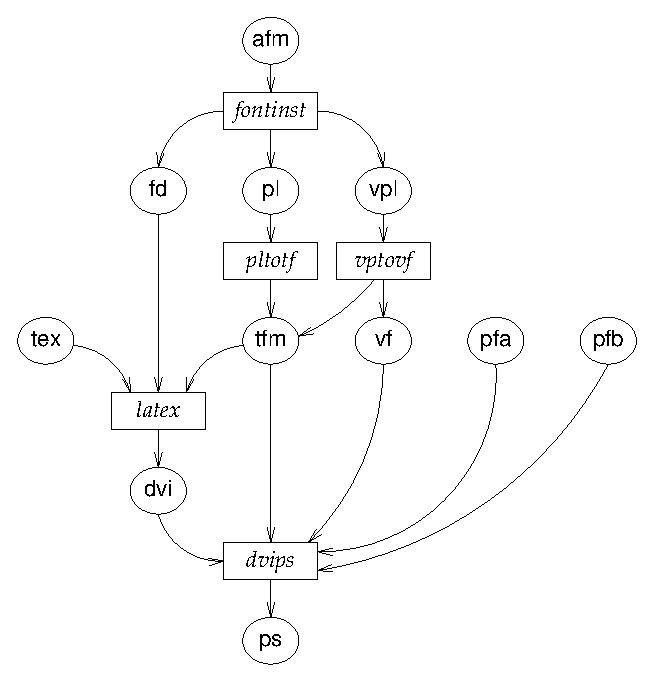
\includegraphics[width=0.40\textwidth]{./fig/exemploFig1}
  \caption{Uma figura típica.}
  \label{fig:exemploFig1}
 \end{figure}
\end{Verbatim}

Ao se usar o compilador \LaTeX, as figuras podem estar nos formatos \textit{eps} e \textit{ps}. Ao se usar o PDF\LaTeX, as figuras podem estar nos formatos \textit{png}, \textit{jpg}, \textit{pdf} e \textit{mps}. A classe \verb|graphicx| também pode ser usada para a inclusão de figuras, nos formatos listados, ao se usar o PDF\LaTeX. Os comandos necessários são os mesmos ao se incluir figuras ao se usar o compilador \LaTeX. O uso do comando \verb|\includegraphics| faz com com que PDF\LaTeX\ procure primeiro por figuras com extensão \textit{pdf}, depois \textit{jpg}, depois \textit{mps} e por último \textit{png}. Aqui também não é necessário especificar a extensão do arquivo.

Para a inclusão das figuras \ref{fig:exemploFig1} à \ref{fig:exemploFig3} os comandos usados, tanto no \LaTeX\ quanto no PDF\LaTeX, seriam os mesmos. É claro que em cada caso devem estar disponíveis as figuras nos formatos suportados por cada compilador. Por exemplo, para a inclusão da figura \ref{fig:exemploFig3} foram usados:
\begin{Verbatim}
 \begin{figure}[H]
  \centering
  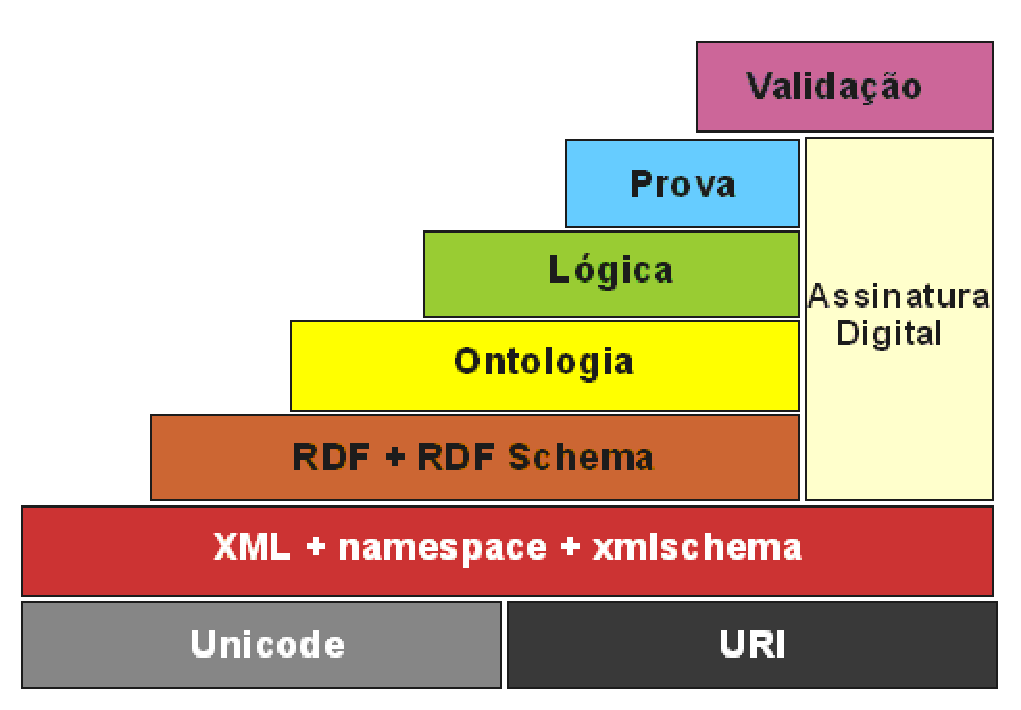
\includegraphics[width=0.40\textwidth]{./fig/exemploFig3}
  \caption{Figura incluída no texto com a classe graphicx.}
  \label{fig:exemploFig3}
\end{figure}
\end{Verbatim}

\begin{figure}[H]
 \centering
  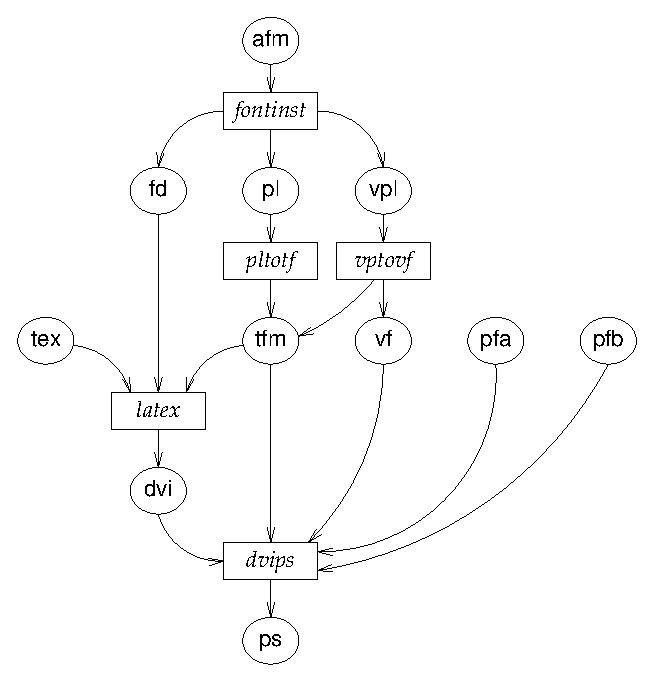
\includegraphics[width=0.40\textwidth]{./fig/exemploFig1}
 \caption{Uma figura típica.}
 \label{fig:exemploFig1}
\end{figure}

\begin{figure}[H]
 \centering
 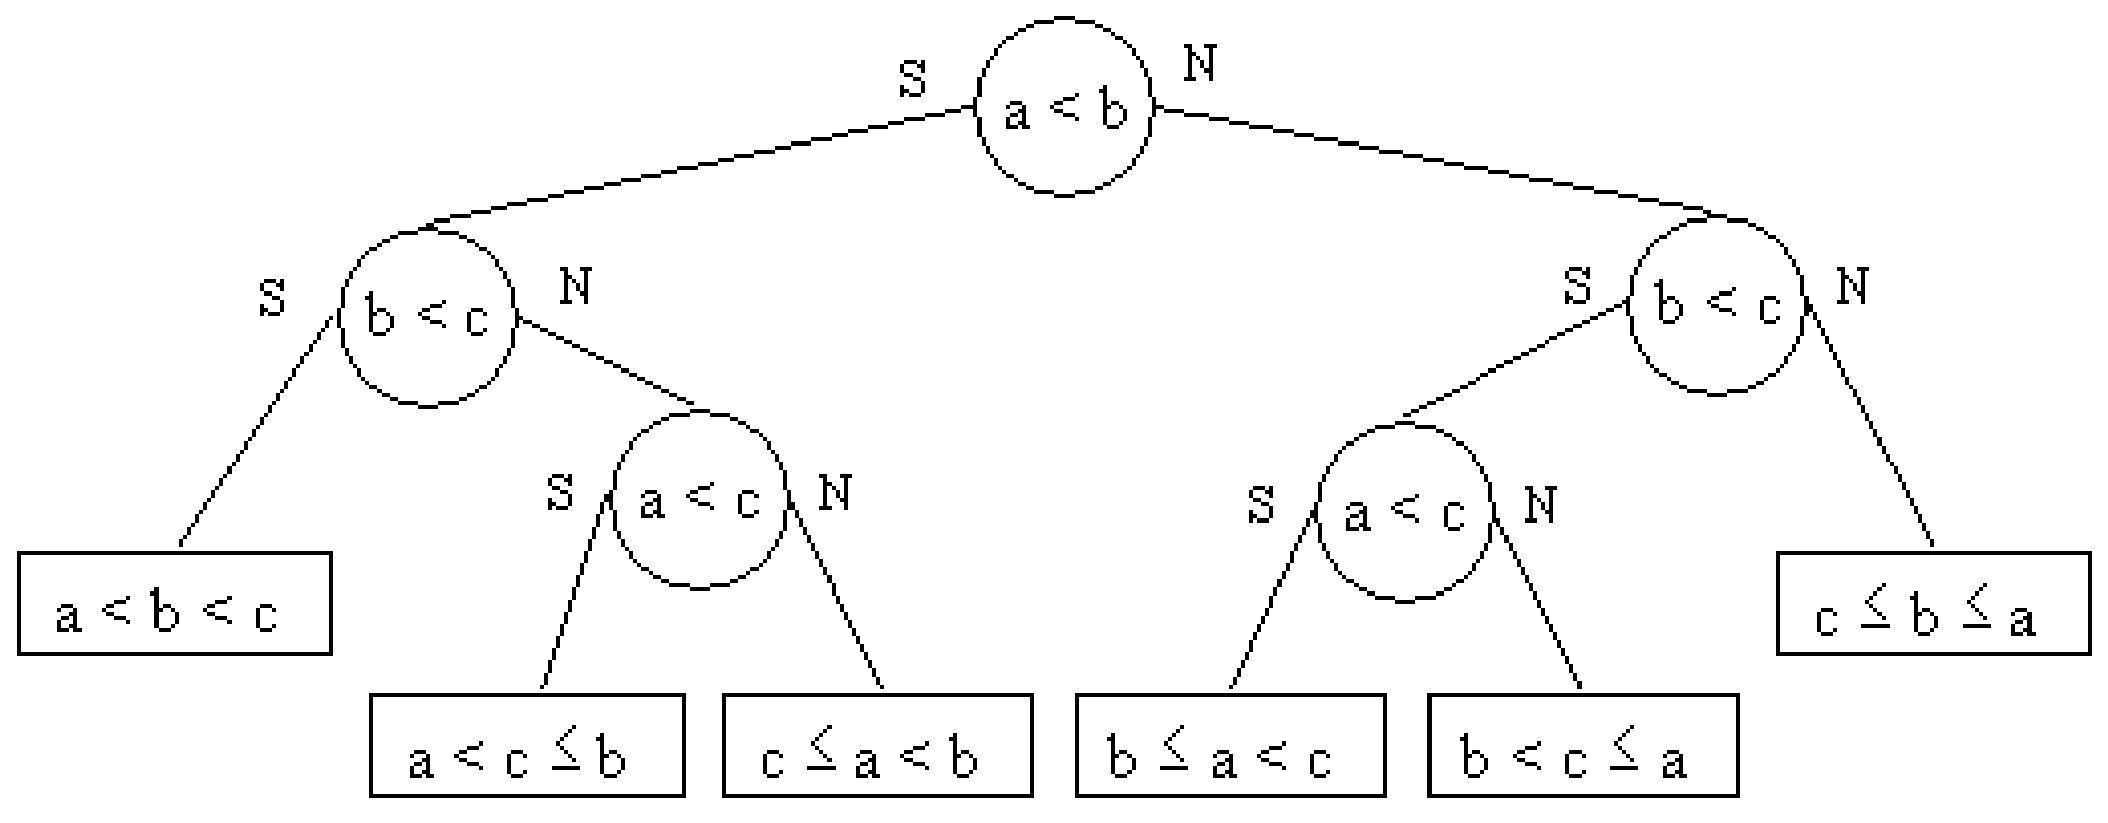
\includegraphics[width=0.30\textwidth]{./fig/exemploFig2}
 \caption{Esta figura é um exemplo de um rótulo de figura que ocupa mais de uma linha, devendo ser identado e justificado.}
 \label{fig:exemploFig2}
\end{figure}

\begin{figure}[H]
 \centering
  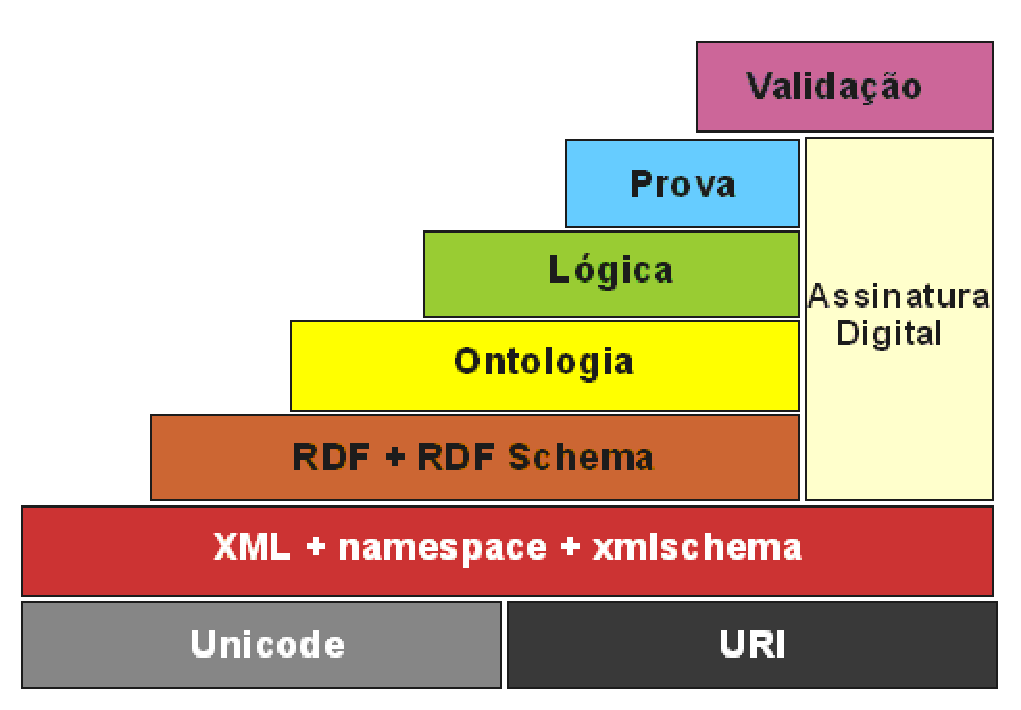
\includegraphics[width=0.40\textwidth]{./fig/exemploFig3}
  \caption{Figura incluída no texto com a classe graphicx.}
 \label{fig:exemploFig3}
\end{figure}

\subsection{Subfiguras}
\label{subsec:subfigs} 
A classe \verb|subfigure| pode ser usada para a inclusão de figuras dentro de figuras (consulte a documentação da classe para maiores detalhes). Por exemplo, a Figura \ref{fig:subfiguras} contém duas subfiguras. Estas podem ser referencidas por rótulos independentes, ou seja, podem ser referenciadas como Figuras \ref{subfig:ex1} e \ref{subfig:ex2} ou Subfiguras \subref{subfig:ex1} e \subref{subfig:ex2}.

A figura \ref{fig:subfiguras} foi incluída com os comandos listados a seguir. Observe que há rótulos independentes para cada uma das subfiguras e um rótulo geral para a figura, os quais podem ser todos referenciados.
\begin{Verbatim}
\begin{figure}[h]
 \centering
  \subfigure[Primeira subfigura.]
   {
    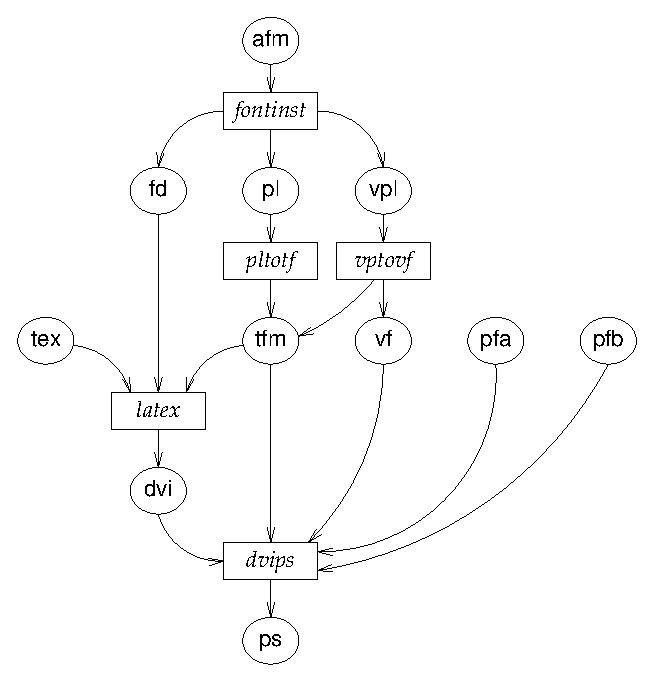
\includegraphics[width=0.35\textwidth]{./fig/exemploFig1}
    \label{subfig:ex1}
   } \qquad
  \subfigure[Segunda subfigura (um pedaço).]
   {
    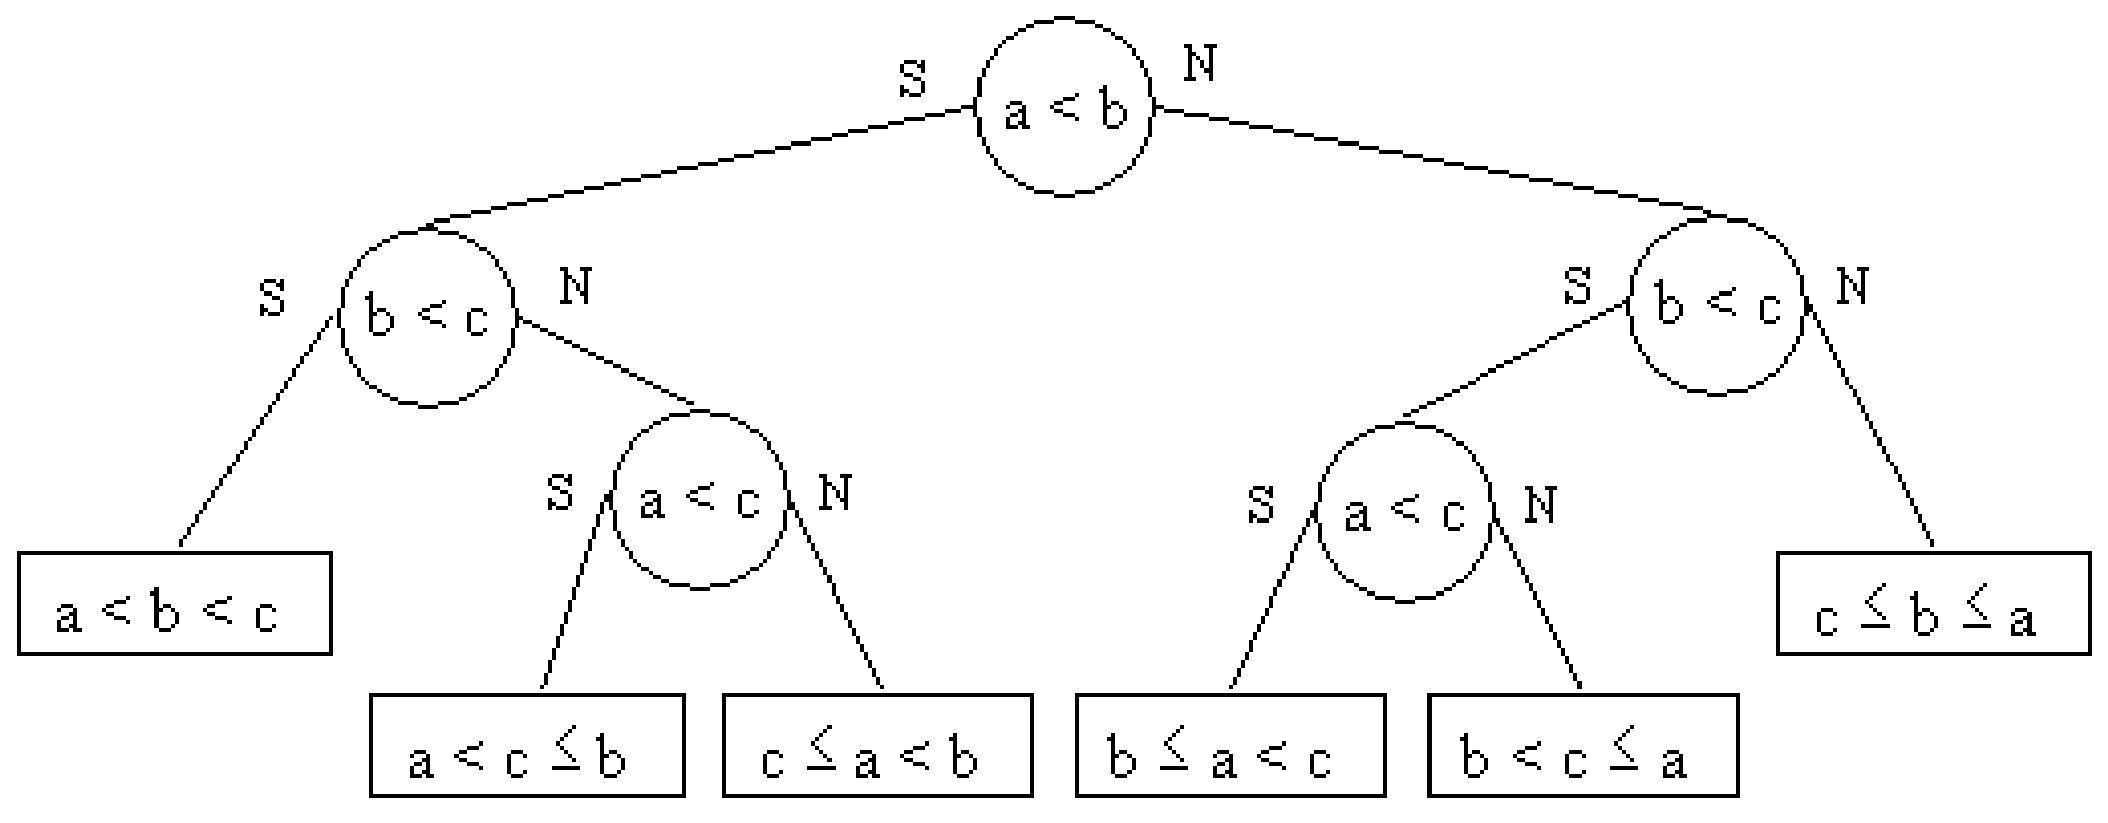
\includegraphics[width=0.30\textwidth]{./fig/exemploFig2}
    \label{subfig:ex2}
   }
   \caption{{\subref{subfig:ex1}} e {\subref{subfig:ex2}} representam
             dois exemplos do uso de subfiguras dentro de uma única
             figura.}
  \label{fig:subfiguras}
\end{figure}
\end{Verbatim}
 Caso uma subfiguras não tenha rótulo, para evitar que o apenas o número da mesma apareça na Lista de Figuras, use o comando \verb|\subfigure[][]|.  Caso uma subfigura tenha rótulo e deseja-se evitar que a mesma apareça na Lista de Figuras, use o comando \verb|\subfigure[][Rótulo]|.
%% - - - - - - - - - - - - - - - - - - - - - - - - - - - - - - - - - - -
\section{Tabelas}
\label{sec:tabs} 
Em tabelas, deve-se evitar usar cor de fundo diferente do branco e o uso de linhas grossas ou duplas. Ao relatar dados empíricos, não se deve usar mais dígitos decimais do aqueles que possam ser garantidos pela sua precisão e reprodutibilidade. Rótulos de tabelas devem ser colocados
antes das mesmas (veja a Tabela \ref{tab:MarcMNem}).

\begin{table*}[hp]
\centering
\caption{Conteúdo do diretório \cite{Mar2004} }
\label{tab:MarcMNem} 
\begin{tabular}{|c|c|c|c|c|c|c|}
\hline Tag & Comprimento & Início &   & Tag & Comprimento & Início \\ 
\hline 001 & 0020 & 00000 && 100 & 0032 & 00235\\ 
\hline 003 & 0004 & 00020 && 245 & 0087 & 00267\\ 
\hline 005 & 0017 & 00024 && 246 & 0036 & 00354\\ 
\hline 008 & 0041 & 00041 && 250 & 0012 & 00390\\ 
\hline 010 & 0024 & 00082 && 260 & 0037 & 00402\\ 
\hline 020 & 0025 & 00106 && 300 & 0029 & 00439\\ 
\hline 020 & 0044 & 00131 && 500 & 0042 & 00468\\ 
\hline 040 & 0018 & 00175 && 520 & 0220 & 00510\\ 
\hline 050 & 0024 & 00193 && 650 & 0033 & 00730\\ 
\hline 082 & 0018 & 00217 && 650 & 0012 & 00763\\ 
\hline 
\end{tabular} 
\end{table*}

%% - - - - - - - - - - - - - - - - - - - - - - - - - - - - - - - - - - -
\section{Algoritmos}
\label{sec:algor} 
Algoritmos devem ser representados no formato do Algoritmo \ref{alg:poten}, que foi descrito com o uso da classe \textsf{algorithm2e}. A rigor não é obrigatório o uso dessa classe, contudo o uso da mesma permite que seja gerada automaticamente uma lista de algoritmos logo após o sumário.

\medskip
\begin{center}
\begin{minipage}{0.92\textwidth}
\begin{algorithm2e}[H]
 \DontPrintSemicolon
 \LinesNumbered
 \SetAlgoLined
 \BlankLine
 \Entrada{vetor $A[i\,.\,.\,j]$, inteiros não negativos $i$ e $j$.}
 \Saida{vetor $A[i\,.\,.\,j]$ ordenado.}
 \BlankLine
 $n \leftarrow j - i$.\;
 \eSe{$(n<4)$}
   {Ordene com $\leq 3$ comparações.}
   {Divida $A$ em $\lceil\sqrt{n}\,\,\rceil$ subvetores de comprimento máximo $\lfloor\sqrt{n}\,\rfloor$.\;
    Aplique $MSR$ a cada um dos subvetores.\;
    Intercale os subvetores.\;}
\caption{$MSR(A,i,j)$ \label {alg:poten}}
\end{algorithm2e}
\end{minipage}
\end{center}

%% - - - - - - - - - - - - - - - - - - - - - - - - - - - - - - - - - - -
\section{Códigos de Programa}
\label{sec:progs} 
Códigos de programa podem ser importados, mantendo-se a formatação original, conforme se pode ver no exemplo do Código \ref{code:prog1}. Este exemplo usa o ambiente \textsf{codigo}, definido na classe \textsf{inf-ufg}, que permite que uma lista de programas seja gerada automaticamente logo após o sumário.
\begin{center}
 \begin{minipage}{0.7\textwidth}
  \begin{codigo}[H]
   \small
   \VerbatimInput[xleftmargin=10mm,numbers=left,obeytabs=true]{./prog/insertionsort.c}
   \caption{\texttt{insertionsort()} }
   \label{code:prog1}
  \end{codigo}
 \end{minipage}
\end{center}

%% - - - - - - - - - - - - - - - - - - - - - - - - - - - - - - - - - - -
\section{Teoremas, Corolários e Demonstrações}
\label{sec:teor}
 O uso do ambiente \textsf{theorem} permite a escrita de teoremas, como no exemplo a seguir:
\begin{verbatim}
\begin{theorem}[Pitágoras]
Em todo triângulo retângulo o quadrado do comprimento
da hipotenusa é igual a soma dos quadrados dos
comprimentos dos catetos.
\end{theorem}
\end{verbatim}

O resultado é o mostrado a seguir:

\begin{theorem}[Pitágoras]
Em todo triângulo retângulo o quadrado do comprimento da hipotenusa é igual a soma dos quadrados dos comprimentos dos catetos.
\end{theorem}

Da mesma forma pode-se usar o ambiente \textsf{proof} para demonstrações de teoremas:
\begin{verbatim}
\begin{proof}
Para demonstrar o Teorema de Pitágoras \dots
\end{proof}
\end{verbatim}

Neste caso, o resultado é:
\begin{proof}
Para demonstrar o Teorema de Pitágoras \dots
\end{proof}

Além desses dois ambientes, estão definidos os ambientes \textsf{definition} (Definição), \textsf{corollary} (Corolário), \textsf{lemma} (Lema)), \textsf{proposition} (Proposição), \textsf{comment} (Observação).

%% - - - - - - - - - - - - - - - - - - - - - - - - - - - - - - - - - - -
\section{Citações Longas}
\label{sec:citacoes}

Segundo as normas da ABNT, uma citação longa (mais de 3 linhas) deve seguir uma formação especial. Para tanto foi criado o ambiente \verb|citacao|, o qual é baseado no ambiente de mesmo nome definido pelo grupo ABNTex \cite{abnt-classe-doc}:
\begin{citacao}
Uma citação longa (mais de 3 linhas) deve vir em parágrafo separado,
com recuo de 4cm da margem esquerda, em fonte menor, sem as aspas
\cite[4.4]{NBR10520:2001} e com espaçamento simples \cite[5.3]{NBR14724:2001}.
Uma regra de como fazer citações em geral não é simples. É prudente
ler \cite{NBR10520:2001} se você optar for fazer uso freqüente de citações.
Para satisfazer às exigências tipográficas que a norma pede para
citações longas, use o ambiente citacao.
\end{citacao}

Este exemplo de citação longa foi produzido com o uso do ambiente \verb|citacao|, como descrito logo a seguir:

\begin{verbatim}
\begin{citacao}
Uma citação longa (mais de 3 linhas) deve vir em parágrafo
separado, com recuo de 4cm da margem esquerda, em fonte menor,
sem as aspas \cite[4.4]{NBR10520:2001} e com espaçamento
simples \cite[5.3]{NBR14724:2001}. Uma regra de como fazer
citações em geral não é simples. É prudente ler
\cite{NBR10520:2001} se você optar for fazer uso freqüente
de citações. Para satisfazer às exigências tipográficas que a
norma pede para citações longas, use o ambiente citacao.
\end{citacao}
\end{verbatim}

%% - - - - - - - - - - - - - - - - - - - - - - - - - - - - - - - - - - -
\section{Referências Bibliográficas}
\label{sec:refs} 
Esta seção mostra exemplos de uso de referências bibliográficas com \BibTeX{} e
do comando \verb|\cite|.  Muitas das entradas listadas na página~\pageref{ref-bib}
foram obtidas de: \href{http://liinwww.ira.uka.de/bibliography/index.html}{http://liinwww.ira.uka.de/bibliography/index.html}.  Outro grande repositório de referências já em formato \BibTeX{} está disponível em:
\href{http://www.math.utah.edu/~beebe/bibliographies.html}{http://www.math.utah.edu/~beebe/bibliographies.html}.

As referências bibliográficas devem ser não ambíguas e uniformes. Recomenda-se usar números entre colchetes, como por exemplo \cite{SmiJon1999}, \cite{Knu1989} e \cite{LeeSwi2002}.
O comando \verb|\nocite| não produz texto, mas permite que a entrada
seja incluída nas referências. Por exemplo, o comando \verb|\nocite{Ber1970}| gera na lista de referências bibliográficas a entrada referente à chave \textsf{Ber1970}, mas não inclui nenhuma referência no texto. O comando \verb|\nocite{*}| faz com que todas as entradas do arquivo de dados do \BibTeX{} sejam incluídas nas referências. \nocite{Ber1970}

Existem vários livros sobre \LaTeX{}, como \cite{Bue1990,Hah1991,KopDal1995}, embora os mais famosos sejam sem dúvida \cite{Lam1996} e \cite{GooMitSam1994}. Para converter documentos \LaTeX{} para HTML veja \cite[pg.1--10]{Dra1994}.




%------------------------------------------------------------ BIBLIOGRAFIA %
\cleardoublepage
\nocite{*} %%% Retire esta linha para gerar a bibliografia com apenas as
           %%% referências usadas no seu texto!
\arial
\bibliography{./bib/modelo-tese} %%% Nomes dos seus arquivos .bib
\label{ref-bib}

%--------------------------------------------------------------- APÊNDICES %
\apendices

\chapter{Exemplo de um Apêndice}
\label{apend:1}
Apêndicess são iniciados com o comando \verb|\apendices|.
Apêndicess são iniciados com o comando \verb|\apendices|.
Apêndicess são iniciados com o comando \verb|\apendices|.
Apêndicess são iniciados com o comando \verb|\apendices|.
Apêndicess são iniciados com o comando \verb|\apendices|.
Apêndicess são iniciados com o comando \verb|\apendices|.
Apêndicess são iniciados com o comando \verb|\apendices|.
Apêndicess são iniciados com o comando \verb|\apendices|.
Apêndicess são iniciados com o comando \verb|\apendices|.
Apêndicess são iniciados com o comando \verb|\apendices|.
Apêndicess são iniciados com o comando \verb|\apendices|.
Apêndicess são iniciados com o comando \verb|\apendices|.
Apêndicess são iniciados com o comando \verb|\apendices|.
Apêndicess são iniciados com o comando \verb|\apendices|.
Apêndicess são iniciados com o comando \verb|\apendices|.
Apêndicess são iniciados com o comando \verb|\apendices|.

Apêndicess são iniciados com o comando \verb|\apendices|.
Apêndicess são iniciados com o comando \verb|\apendices|.
Apêndicess são iniciados com o comando \verb|\apendices|.
Apêndicess são iniciados com o comando \verb|\apendices|.
Apêndicess são iniciados com o comando \verb|\apendices|.
Apêndicess são iniciados com o comando \verb|\apendices|.
Apêndicess são iniciados com o comando \verb|\apendices|.
Apêndicess são iniciados com o comando \verb|\apendices|.
Apêndicess são iniciados com o comando \verb|\apendices|.
Apêndicess são iniciados com o comando \verb|\apendices|.
Apêndicess são iniciados com o comando \verb|\apendices|.
Apêndicess são iniciados com o comando \verb|\apendices|.

Apêndicess são iniciados com o comando \verb|\apendices|.
Apêndicess são iniciados com o comando \verb|\apendices|.
Apêndicess são iniciados com o comando \verb|\apendices|.
Apêndicess são iniciados com o comando \verb|\apendices|.
Apêndicess são iniciados com o comando \verb|\apendices|.
Apêndicess são iniciados com o comando \verb|\apendices|.
Apêndicess são iniciados com o comando \verb|\apendices|.
Apêndicess são iniciados com o comando \verb|\apendices|.
Apêndicess são iniciados com o comando \verb|\apendices|.
Apêndicess são iniciados com o comando \verb|\apendices|.
Apêndicess são iniciados com o comando \verb|\apendices|.
Apêndicess são iniciados com o comando \verb|\apendices|.
Apêndicess são iniciados com o comando \verb|\apendices|.
Apêndicess são iniciados com o comando \verb|\apendices|.

Apêndicess são iniciados com o comando \verb|\apendices|.
Apêndicess são iniciados com o comando \verb|\apendices|.
Apêndicess são iniciados com o comando \verb|\apendices|.
Apêndicess são iniciados com o comando \verb|\apendices|.
Apêndicess são iniciados com o comando \verb|\apendices|.
Apêndicess são iniciados com o comando \verb|\apendices|.
Apêndicess são iniciados com o comando \verb|\apendices|.
Apêndicess são iniciados com o comando \verb|\apendices|.
Apêndicess são iniciados com o comando \verb|\apendices|.
Apêndicess são iniciados com o comando \verb|\apendices|.
Apêndicess são iniciados com o comando \verb|\apendices|.
Apêndicess são iniciados com o comando \verb|\apendices|.
Apêndicess são iniciados com o comando \verb|\apendices|.
Apêndicess são iniciados com o comando \verb|\apendices|.

Apêndicess são iniciados com o comando \verb|\apendices|.
Apêndicess são iniciados com o comando \verb|\apendices|.
Apêndicess são iniciados com o comando \verb|\apendices|.
Apêndicess são iniciados com o comando \verb|\apendices|.
Apêndicess são iniciados com o comando \verb|\apendices|.
Apêndicess são iniciados com o comando \verb|\apendices|.
Apêndicess são iniciados com o comando \verb|\apendices|.
Apêndicess são iniciados com o comando \verb|\apendices|.
Apêndicess são iniciados com o comando \verb|\apendices|.
Apêndicess são iniciados com o comando \verb|\apendices|.
Apêndicess são iniciados com o comando \verb|\apendices|.
Apêndicess são iniciados com o comando \verb|\apendices|.
Apêndicess são iniciados com o comando \verb|\apendices|.
Apêndicess são iniciados com o comando \verb|\apendices|.

Apêndicess são iniciados com o comando \verb|\apendices|.
Apêndicess são iniciados com o comando \verb|\apendices|.
Apêndicess são iniciados com o comando \verb|\apendices|.
Apêndicess são iniciados com o comando \verb|\apendices|.
Apêndicess são iniciados com o comando \verb|\apendices|.
Apêndicess são iniciados com o comando \verb|\apendices|.
Apêndicess são iniciados com o comando \verb|\apendices|.
Apêndicess são iniciados com o comando \verb|\apendices|.
Apêndicess são iniciados com o comando \verb|\apendices|.
Apêndicess são iniciados com o comando \verb|\apendices|.
Apêndicess são iniciados com o comando \verb|\apendices|.
Apêndicess são iniciados com o comando \verb|\apendices|.
Apêndicess são iniciados com o comando \verb|\apendices|.
Apêndicess são iniciados com o comando \verb|\apendices|.

Apêndicess são iniciados com o comando \verb|\apendices|.
Apêndicess são iniciados com o comando \verb|\apendices|.
Apêndicess são iniciados com o comando \verb|\apendices|.
Apêndicess são iniciados com o comando \verb|\apendices|.
Apêndicess são iniciados com o comando \verb|\apendices|.
Apêndicess são iniciados com o comando \verb|\apendices|.
Apêndicess são iniciados com o comando \verb|\apendices|.
Apêndicess são iniciados com o comando \verb|\apendices|.
Apêndicess são iniciados com o comando \verb|\apendices|.
Apêndicess são iniciados com o comando \verb|\apendices|.
Apêndicess são iniciados com o comando \verb|\apendices|.
Apêndicess são iniciados com o comando \verb|\apendices|.
Apêndicess são iniciados com o comando \verb|\apendices|.
Apêndicess são iniciados com o comando \verb|\apendices|.

Apêndicess são iniciados com o comando \verb|\apendices|.
Apêndicess são iniciados com o comando \verb|\apendices|.
Apêndicess são iniciados com o comando \verb|\apendices|.
Apêndicess são iniciados com o comando \verb|\apendices|.
Apêndicess são iniciados com o comando \verb|\apendices|.
Apêndicess são iniciados com o comando \verb|\apendices|.
Apêndicess são iniciados com o comando \verb|\apendices|.
Apêndicess são iniciados com o comando \verb|\apendices|.
Apêndicess são iniciados com o comando \verb|\apendices|.
Apêndicess são iniciados com o comando \verb|\apendices|.
Apêndicess são iniciados com o comando \verb|\apendices|.
Apêndicess são iniciados com o comando \verb|\apendices|.
Apêndicess são iniciados com o comando \verb|\apendices|.
Apêndicess são iniciados com o comando \verb|\apendices|.

Apêndicess são iniciados com o comando \verb|\apendices|.
Apêndicess são iniciados com o comando \verb|\apendices|.
Apêndicess são iniciados com o comando \verb|\apendices|.
Apêndicess são iniciados com o comando \verb|\apendices|.
Apêndicess são iniciados com o comando \verb|\apendices|.
Apêndicess são iniciados com o comando \verb|\apendices|.
Apêndicess são iniciados com o comando \verb|\apendices|.
Apêndicess são iniciados com o comando \verb|\apendices|.
Apêndicess são iniciados com o comando \verb|\apendices|.
Apêndicess são iniciados com o comando \verb|\apendices|.
Apêndicess são iniciados com o comando \verb|\apendices|.
Apêndicess são iniciados com o comando \verb|\apendices|.
Apêndicess são iniciados com o comando \verb|\apendices|.
Apêndicess são iniciados com o comando \verb|\apendices|.

Apêndicess são iniciados com o comando \verb|\apendices|.
Apêndicess são iniciados com o comando \verb|\apendices|.
Apêndicess são iniciados com o comando \verb|\apendices|.
Apêndicess são iniciados com o comando \verb|\apendices|.
Apêndicess são iniciados com o comando \verb|\apendices|.
Apêndicess são iniciados com o comando \verb|\apendices|.
Apêndicess são iniciados com o comando \verb|\apendices|.
Apêndicess são iniciados com o comando \verb|\apendices|.
Apêndicess são iniciados com o comando \verb|\apendices|.
Apêndicess são iniciados com o comando \verb|\apendices|.
Apêndicess são iniciados com o comando \verb|\apendices|.
Apêndicess são iniciados com o comando \verb|\apendices|.
Apêndicess são iniciados com o comando \verb|\apendices|.
Apêndicess são iniciados com o comando \verb|\apendices|.

Apêndicess são iniciados com o comando \verb|\apendices|.
Apêndicess são iniciados com o comando \verb|\apendices|.
Apêndicess são iniciados com o comando \verb|\apendices|.
Apêndicess são iniciados com o comando \verb|\apendices|.
Apêndicess são iniciados com o comando \verb|\apendices|.
Apêndicess são iniciados com o comando \verb|\apendices|.
Apêndicess são iniciados com o comando \verb|\apendices|.
Apêndicess são iniciados com o comando \verb|\apendices|.
Apêndicess são iniciados com o comando \verb|\apendices|.
Apêndicess são iniciados com o comando \verb|\apendices|.
Apêndicess são iniciados com o comando \verb|\apendices|.
Apêndicess são iniciados com o comando \verb|\apendices|.
Apêndicess são iniciados com o comando \verb|\apendices|.
Apêndicess são iniciados com o comando \verb|\apendices|.

Apêndicess são iniciados com o comando \verb|\apendices|.
Apêndicess são iniciados com o comando \verb|\apendices|.
Apêndicess são iniciados com o comando \verb|\apendices|.
Apêndicess são iniciados com o comando \verb|\apendices|.
Apêndicess são iniciados com o comando \verb|\apendices|.
Apêndicess são iniciados com o comando \verb|\apendices|.
Apêndicess são iniciados com o comando \verb|\apendices|.
Apêndicess são iniciados com o comando \verb|\apendices|.
Apêndicess são iniciados com o comando \verb|\apendices|.
Apêndicess são iniciados com o comando \verb|\apendices|.
Apêndicess são iniciados com o comando \verb|\apendices|.
Apêndicess são iniciados com o comando \verb|\apendices|.
Apêndicess são iniciados com o comando \verb|\apendices|.
Apêndicess são iniciados com o comando \verb|\apendices|.

Apêndicess são iniciados com o comando \verb|\apendices|.
Apêndicess são iniciados com o comando \verb|\apendices|.
Apêndicess são iniciados com o comando \verb|\apendices|.
Apêndicess são iniciados com o comando \verb|\apendices|.
Apêndicess são iniciados com o comando \verb|\apendices|.
Apêndicess são iniciados com o comando \verb|\apendices|.
Apêndicess são iniciados com o comando \verb|\apendices|.
Apêndicess são iniciados com o comando \verb|\apendices|.
Apêndicess são iniciados com o comando \verb|\apendices|.
Apêndicess são iniciados com o comando \verb|\apendices|.
Apêndicess são iniciados com o comando \verb|\apendices|.
Apêndicess são iniciados com o comando \verb|\apendices|.
Apêndicess são iniciados com o comando \verb|\apendices|.
Apêndicess são iniciados com o comando \verb|\apendices|.

Apêndicess são iniciados com o comando \verb|\apendices|.
Apêndicess são iniciados com o comando \verb|\apendices|.
Apêndicess são iniciados com o comando \verb|\apendices|.
Apêndicess são iniciados com o comando \verb|\apendices|.
Apêndicess são iniciados com o comando \verb|\apendices|.
Apêndicess são iniciados com o comando \verb|\apendices|.
Apêndicess são iniciados com o comando \verb|\apendices|.
Apêndicess são iniciados com o comando \verb|\apendices|.
Apêndicess são iniciados com o comando \verb|\apendices|.
Apêndicess são iniciados com o comando \verb|\apendices|.
Apêndicess são iniciados com o comando \verb|\apendices|.
Apêndicess são iniciados com o comando \verb|\apendices|.
Apêndicess são iniciados com o comando \verb|\apendices|.
Apêndicess são iniciados com o comando \verb|\apendices|.
\chapter{Exemplo de Outro Apêndice}
\label{apend:2}
Texto do Apêndice~\ref{apend:2}.

Apêndices são iniciados com o comando \verb|\apendices|.
Apêndices são iniciados com o comando \verb|\apendices|.
Apêndices são iniciados com o comando \verb|\apendices|.
Apêndices são iniciados com o comando \verb|\apendices|.
Apêndices são iniciados com o comando \verb|\apendices|.
Apêndices são iniciados com o comando \verb|\apendices|.
Apêndices são iniciados com o comando \verb|\apendices|.
Apêndices são iniciados com o comando \verb|\apendices|.
Apêndices são iniciados com o comando \verb|\apendices|.
Apêndices são iniciados com o comando \verb|\apendices|.
Apêndices são iniciados com o comando \verb|\apendices|.
Apêndices são iniciados com o comando \verb|\apendices|.
Apêndices são iniciados com o comando \verb|\apendices|.
Apêndices são iniciados com o comando \verb|\apendices|.
Apêndices são iniciados com o comando \verb|\apendices|.
Apêndices são iniciados com o comando \verb|\apendices|.

Apêndices são iniciados com o comando \verb|\apendices|.
Apêndices são iniciados com o comando \verb|\apendices|.
Apêndices são iniciados com o comando \verb|\apendices|.
Apêndices são iniciados com o comando \verb|\apendices|.
Apêndices são iniciados com o comando \verb|\apendices|.
Apêndices são iniciados com o comando \verb|\apendices|.
Apêndices são iniciados com o comando \verb|\apendices|.
Apêndices são iniciados com o comando \verb|\apendices|.
Apêndices são iniciados com o comando \verb|\apendices|.
Apêndices são iniciados com o comando \verb|\apendices|.
Apêndices são iniciados com o comando \verb|\apendices|.
Apêndices são iniciados com o comando \verb|\apendices|.

Apêndices são iniciados com o comando \verb|\apendices|.
Apêndices são iniciados com o comando \verb|\apendices|.
Apêndices são iniciados com o comando \verb|\apendices|.
Apêndices são iniciados com o comando \verb|\apendices|.
Apêndices são iniciados com o comando \verb|\apendices|.
Apêndices são iniciados com o comando \verb|\apendices|.
Apêndices são iniciados com o comando \verb|\apendices|.
Apêndices são iniciados com o comando \verb|\apendices|.
Apêndices são iniciados com o comando \verb|\apendices|.
Apêndices são iniciados com o comando \verb|\apendices|.
Apêndices são iniciados com o comando \verb|\apendices|.
Apêndices são iniciados com o comando \verb|\apendices|.
Apêndices são iniciados com o comando \verb|\apendices|.
Apêndices são iniciados com o comando \verb|\apendices|.

Apêndices são iniciados com o comando \verb|\apendices|.
Apêndices são iniciados com o comando \verb|\apendices|.
Apêndices são iniciados com o comando \verb|\apendices|.
Apêndices são iniciados com o comando \verb|\apendices|.
Apêndices são iniciados com o comando \verb|\apendices|.
Apêndices são iniciados com o comando \verb|\apendices|.
Apêndices são iniciados com o comando \verb|\apendices|.
Apêndices são iniciados com o comando \verb|\apendices|.
Apêndices são iniciados com o comando \verb|\apendices|.
Apêndices são iniciados com o comando \verb|\apendices|.
Apêndices são iniciados com o comando \verb|\apendices|.
Apêndices são iniciados com o comando \verb|\apendices|.
Apêndices são iniciados com o comando \verb|\apendices|.
Apêndices são iniciados com o comando \verb|\apendices|.

Apêndices são iniciados com o comando \verb|\apendices|.
Apêndices são iniciados com o comando \verb|\apendices|.
Apêndices são iniciados com o comando \verb|\apendices|.
Apêndices são iniciados com o comando \verb|\apendices|.
Apêndices são iniciados com o comando \verb|\apendices|.
Apêndices são iniciados com o comando \verb|\apendices|.
Apêndices são iniciados com o comando \verb|\apendices|.
Apêndices são iniciados com o comando \verb|\apendices|.
Apêndices são iniciados com o comando \verb|\apendices|.
Apêndices são iniciados com o comando \verb|\apendices|.
Apêndices são iniciados com o comando \verb|\apendices|.
Apêndices são iniciados com o comando \verb|\apendices|.
Apêndices são iniciados com o comando \verb|\apendices|.
Apêndices são iniciados com o comando \verb|\apendices|.

Apêndices são iniciados com o comando \verb|\apendices|.
Apêndices são iniciados com o comando \verb|\apendices|.
Apêndices são iniciados com o comando \verb|\apendices|.
Apêndices são iniciados com o comando \verb|\apendices|.
Apêndices são iniciados com o comando \verb|\apendices|.
Apêndices são iniciados com o comando \verb|\apendices|.
Apêndices são iniciados com o comando \verb|\apendices|.
Apêndices são iniciados com o comando \verb|\apendices|.
Apêndices são iniciados com o comando \verb|\apendices|.
Apêndices são iniciados com o comando \verb|\apendices|.
Apêndices são iniciados com o comando \verb|\apendices|.
Apêndices são iniciados com o comando \verb|\apendices|.
Apêndices são iniciados com o comando \verb|\apendices|.
Apêndices são iniciados com o comando \verb|\apendices|.

Apêndices são iniciados com o comando \verb|\apendices|.
Apêndices são iniciados com o comando \verb|\apendices|.
Apêndices são iniciados com o comando \verb|\apendices|.
Apêndices são iniciados com o comando \verb|\apendices|.
Apêndices são iniciados com o comando \verb|\apendices|.
Apêndices são iniciados com o comando \verb|\apendices|.
Apêndices são iniciados com o comando \verb|\apendices|.
Apêndices são iniciados com o comando \verb|\apendices|.
Apêndices são iniciados com o comando \verb|\apendices|.
Apêndices são iniciados com o comando \verb|\apendices|.
Apêndices são iniciados com o comando \verb|\apendices|.
Apêndices são iniciados com o comando \verb|\apendices|.
Apêndices são iniciados com o comando \verb|\apendices|.
Apêndices são iniciados com o comando \verb|\apendices|.

Apêndices são iniciados com o comando \verb|\apendices|.
Apêndices são iniciados com o comando \verb|\apendices|.
Apêndices são iniciados com o comando \verb|\apendices|.
Apêndices são iniciados com o comando \verb|\apendices|.
Apêndices são iniciados com o comando \verb|\apendices|.
Apêndices são iniciados com o comando \verb|\apendices|.
Apêndices são iniciados com o comando \verb|\apendices|.
Apêndices são iniciados com o comando \verb|\apendices|.
Apêndices são iniciados com o comando \verb|\apendices|.
Apêndices são iniciados com o comando \verb|\apendices|.
Apêndices são iniciados com o comando \verb|\apendices|.
Apêndices são iniciados com o comando \verb|\apendices|.
Apêndices são iniciados com o comando \verb|\apendices|.
Apêndices são iniciados com o comando \verb|\apendices|.

Apêndices são iniciados com o comando \verb|\apendices|.
Apêndices são iniciados com o comando \verb|\apendices|.
Apêndices são iniciados com o comando \verb|\apendices|.
Apêndices são iniciados com o comando \verb|\apendices|.
Apêndices são iniciados com o comando \verb|\apendices|.
Apêndices são iniciados com o comando \verb|\apendices|.
Apêndices são iniciados com o comando \verb|\apendices|.
Apêndices são iniciados com o comando \verb|\apendices|.
Apêndices são iniciados com o comando \verb|\apendices|.
Apêndices são iniciados com o comando \verb|\apendices|.
Apêndices são iniciados com o comando \verb|\apendices|.
Apêndices são iniciados com o comando \verb|\apendices|.
Apêndices são iniciados com o comando \verb|\apendices|.
Apêndices são iniciados com o comando \verb|\apendices|.

Apêndices são iniciados com o comando \verb|\apendices|.
Apêndices são iniciados com o comando \verb|\apendices|.
Apêndices são iniciados com o comando \verb|\apendices|.
Apêndices são iniciados com o comando \verb|\apendices|.
Apêndices são iniciados com o comando \verb|\apendices|.
Apêndices são iniciados com o comando \verb|\apendices|.
Apêndices são iniciados com o comando \verb|\apendices|.
Apêndices são iniciados com o comando \verb|\apendices|.
Apêndices são iniciados com o comando \verb|\apendices|.
Apêndices são iniciados com o comando \verb|\apendices|.
Apêndices são iniciados com o comando \verb|\apendices|.
Apêndices são iniciados com o comando \verb|\apendices|.
Apêndices são iniciados com o comando \verb|\apendices|.
Apêndices são iniciados com o comando \verb|\apendices|.

Apêndices são iniciados com o comando \verb|\apendices|.
Apêndices são iniciados com o comando \verb|\apendices|.
Apêndices são iniciados com o comando \verb|\apendices|.
Apêndices são iniciados com o comando \verb|\apendices|.
Apêndices são iniciados com o comando \verb|\apendices|.
Apêndices são iniciados com o comando \verb|\apendices|.
Apêndices são iniciados com o comando \verb|\apendices|.
Apêndices são iniciados com o comando \verb|\apendices|.
Apêndices são iniciados com o comando \verb|\apendices|.
Apêndices são iniciados com o comando \verb|\apendices|.
Apêndices são iniciados com o comando \verb|\apendices|.
Apêndices são iniciados com o comando \verb|\apendices|.
Apêndices são iniciados com o comando \verb|\apendices|.
Apêndices são iniciados com o comando \verb|\apendices|.

Apêndices são iniciados com o comando \verb|\apendices|.
Apêndices são iniciados com o comando \verb|\apendices|.
Apêndices são iniciados com o comando \verb|\apendices|.
Apêndices são iniciados com o comando \verb|\apendices|.
Apêndices são iniciados com o comando \verb|\apendices|.
Apêndices são iniciados com o comando \verb|\apendices|.
Apêndices são iniciados com o comando \verb|\apendices|.
Apêndices são iniciados com o comando \verb|\apendices|.
Apêndices são iniciados com o comando \verb|\apendices|.
Apêndices são iniciados com o comando \verb|\apendices|.
Apêndices são iniciados com o comando \verb|\apendices|.
Apêndices são iniciados com o comando \verb|\apendices|.
Apêndices são iniciados com o comando \verb|\apendices|.
Apêndices são iniciados com o comando \verb|\apendices|.

Apêndices são iniciados com o comando \verb|\apendices|.
Apêndices são iniciados com o comando \verb|\apendices|.
Apêndices são iniciados com o comando \verb|\apendices|.
Apêndices são iniciados com o comando \verb|\apendices|.
Apêndices são iniciados com o comando \verb|\apendices|.
Apêndices são iniciados com o comando \verb|\apendices|.
Apêndices são iniciados com o comando \verb|\apendices|.
Apêndices são iniciados com o comando \verb|\apendices|.
Apêndices são iniciados com o comando \verb|\apendices|.
Apêndices são iniciados com o comando \verb|\apendices|.
Apêndices são iniciados com o comando \verb|\apendices|.
Apêndices são iniciados com o comando \verb|\apendices|.
Apêndices são iniciados com o comando \verb|\apendices|.
Apêndices são iniciados com o comando \verb|\apendices|.

Apêndices são iniciados com o comando \verb|\apendices|.
Apêndices são iniciados com o comando \verb|\apendices|.
Apêndices são iniciados com o comando \verb|\apendices|.
Apêndices são iniciados com o comando \verb|\apendices|.
Apêndices são iniciados com o comando \verb|\apendices|.
Apêndices são iniciados com o comando \verb|\apendices|.
Apêndices são iniciados com o comando \verb|\apendices|.
Apêndices são iniciados com o comando \verb|\apendices|.
Apêndices são iniciados com o comando \verb|\apendices|.
Apêndices são iniciados com o comando \verb|\apendices|.
Apêndices são iniciados com o comando \verb|\apendices|.
Apêndices são iniciados com o comando \verb|\apendices|.
Apêndices são iniciados com o comando \verb|\apendices|.
Apêndices são iniciados com o comando \verb|\apendices|.

\end{document}

%------------------------------------------------------------------------- %
%        F I M   D O  A R Q U I V O :  m o d e l o - t e s e . t e x       %
%------------------------------------------------------------------------- %